\documentclass{beamer}

\usepackage{amsmath}
\usepackage{graphicx}
\usepackage{euler}
\usepackage{verbatim}

%Custom macros go here.

\newcommand{\Ei}{\textrm{Ei}} % Exponential integral
\newcommand{\Eig}{\textrm{Eig}} % Eigenvalues
\newcommand{\e}[0]{\hat{e}} % Unit vector
\newcommand{\norm}[1]{\left|\left|{#1}\right|\right|} % |n|
\newcommand{\fracflat}[2]{\left.{#1}\middle/{#2}\right.} % flat fractions
\newcommand{\flatfrac}[2]{\left.{#1}\middle/{#2}\right.} % flat fractions


\title{The Measurement of Anisotropic Thermal Conductivity in Snow With Needle Probes}
\subtitle{A Thesis Defense}
\author{Joshua Holbrook}
\date{April 4th, 2011}

\begin{document}
\frame{\titlepage}


\begin{frame}
\frametitle{Why Do We Study Snow's Thermal Conductivity?}
\begin{columns}[c]
\column{0.5\textwidth}
     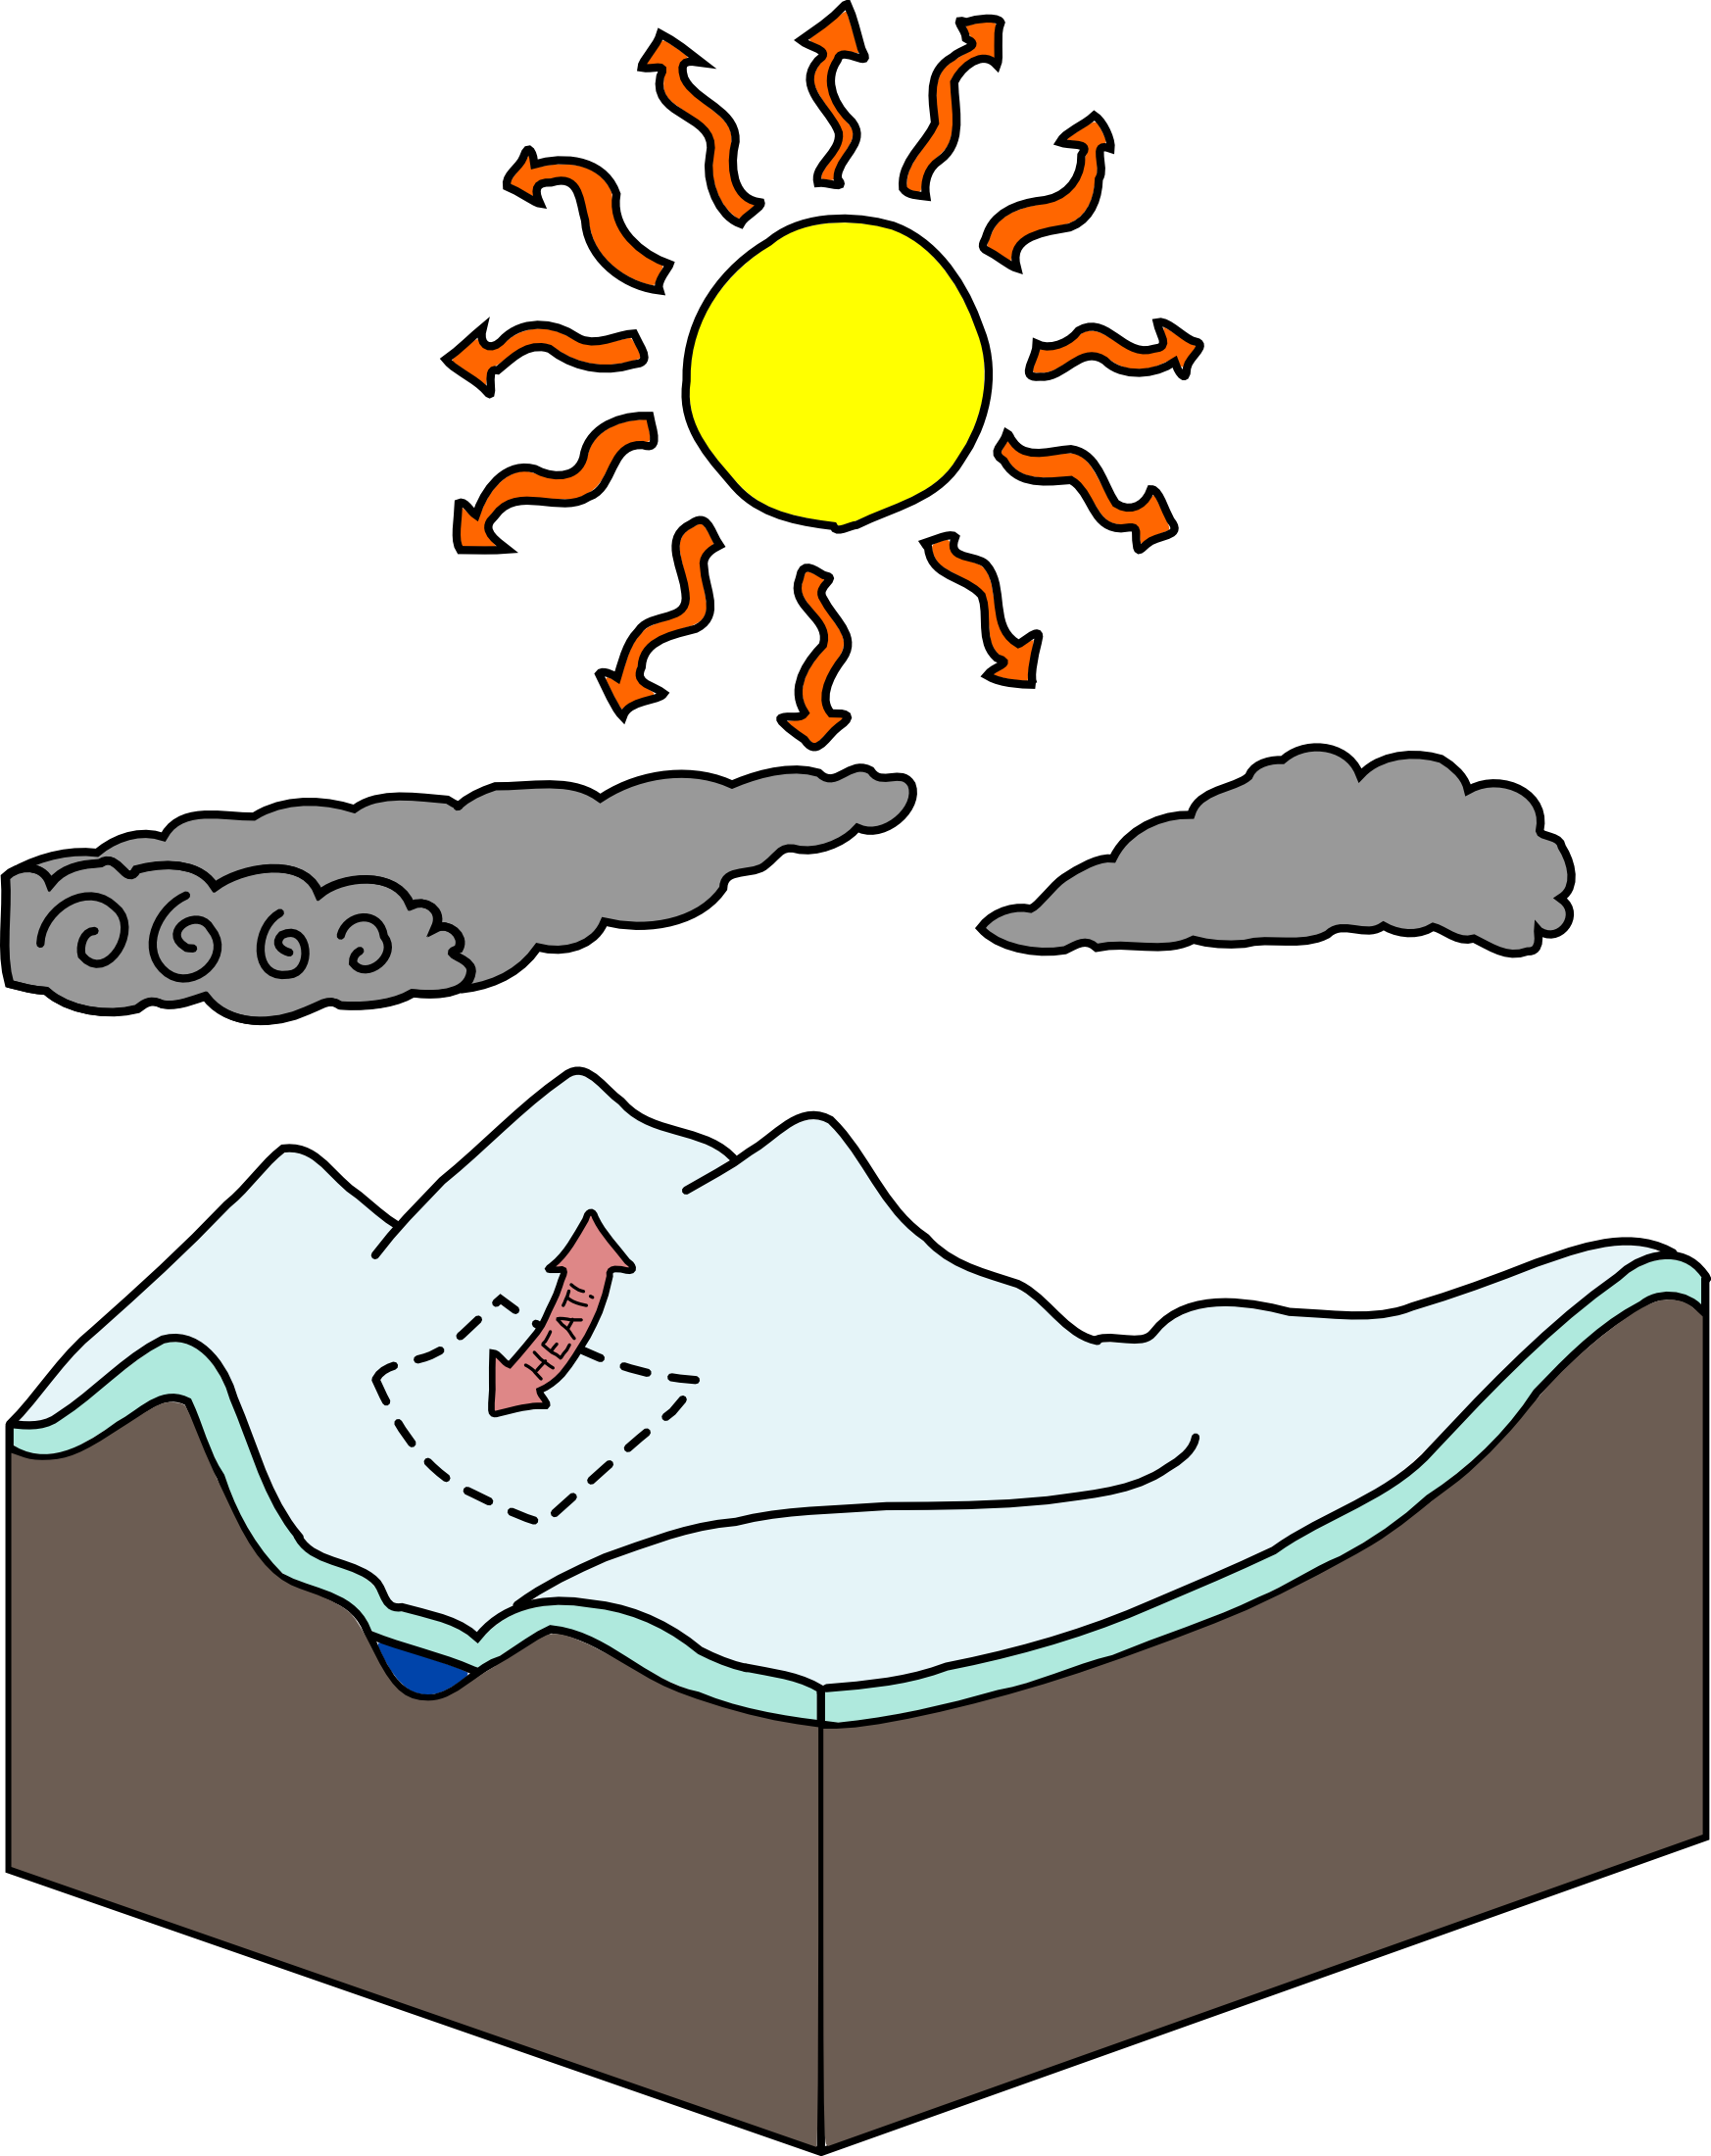
\includegraphics[width=\textwidth]{fig/climate.png}
\column{0.5\textwidth}
    \begin{itemize}
    \item Climatologists want to model Arctic climates.
    \item Heat transfer occurs between the earth and the atmosphere.
    \item Snow gets in the way. It's an \emph{insulating blanket}.
    \end{itemize}
\end{columns}
\end{frame}


\begin{frame}
\frametitle{How Do We Measure Thermal Conductivity?}
    \begin{itemize}
    \item One way is a guarded hot plate.
    \item Steady state 1-D conduction: \(k = \frac{\dot{q}l}{A\Delta T}\)
    \item Guarded hot plates are good for measuring foam boards.
    \item Guarded hot plates aren't exactly ideal for snow.
    \end{itemize}
\end{frame}


\begin{frame}
\frametitle{There HAS to be a better way.}
\begin{columns}[c]
\column{0.5\textwidth}
     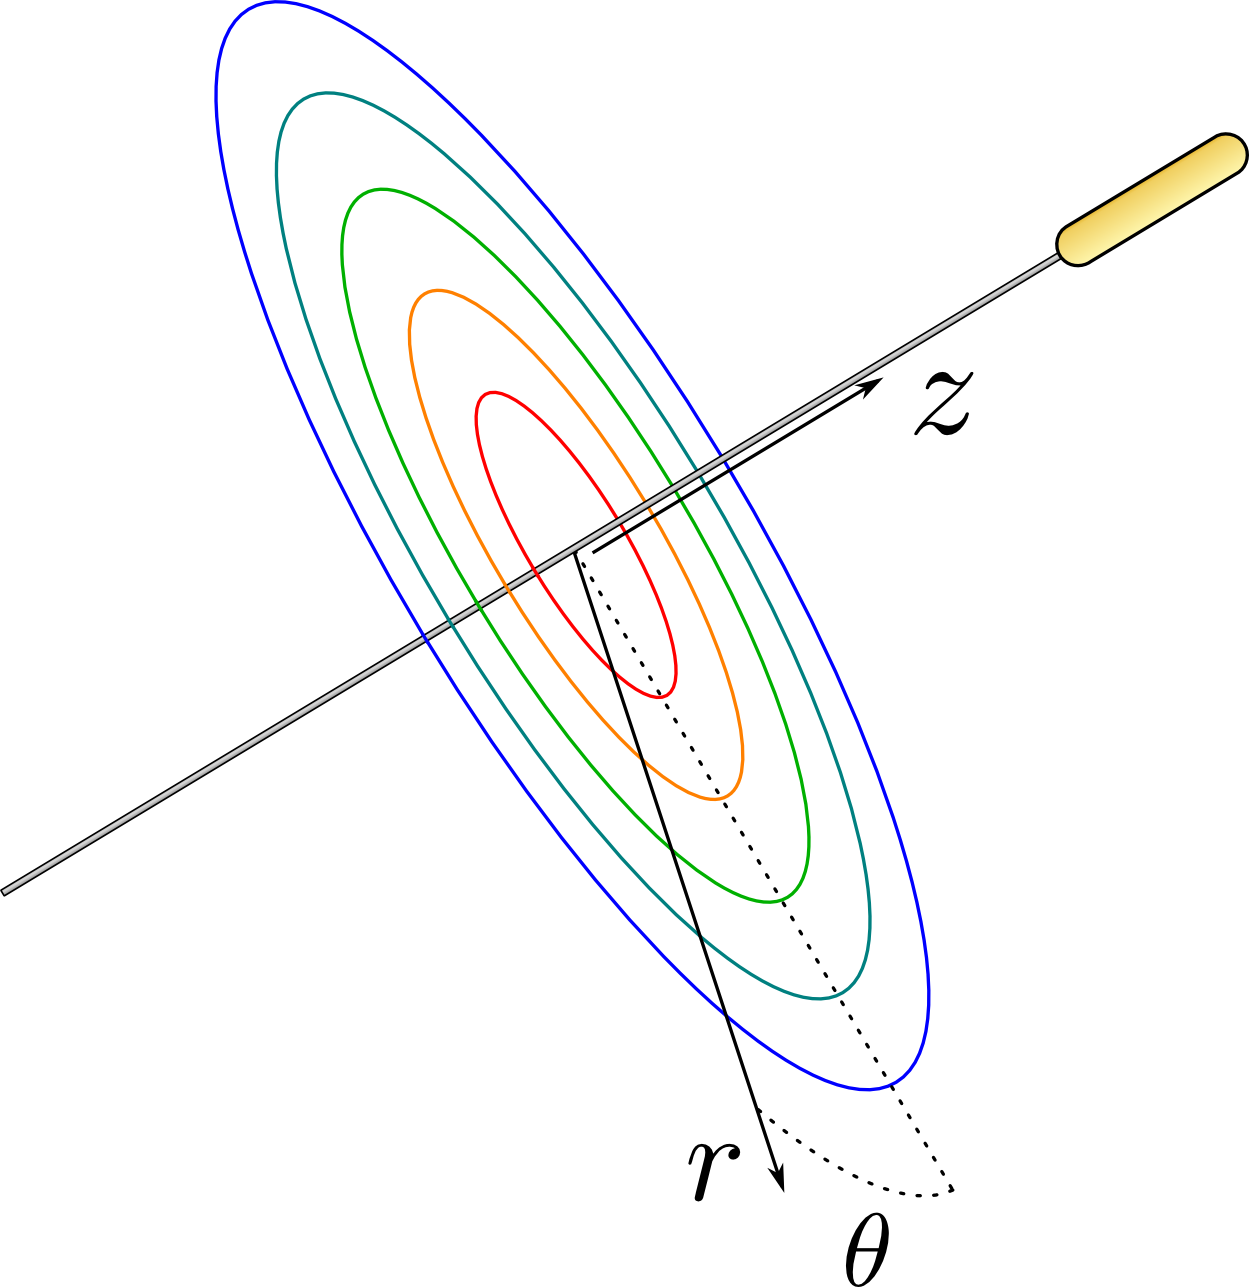
\includegraphics[width=\textwidth]{fig/basic_geometry.png}
\column{0.5\textwidth}
    \begin{itemize}
    \item It's called a needle probe.
    \item It looks something like this.
    \item It does \emph{not} use steady-state conduction.
    \item It depends on a \emph{radial} geometry.
    \item Okay, I'll admit, ``better'' is relative here.
    \end{itemize}
\end{columns}
\end{frame}


\begin{frame}
\frametitle{What Is A Needle Probe, Exactly?}
\begin{columns}[c]
\column{0.5\textwidth}
    \begin{itemize}
    \item Long and thin enough to approximate a line.
    \item Has a thermocouple in the center.
    \item Has heat trace running down most of its length.
    \item This is a drawing of a cross-section of such a needle (The one
          actually used has a slightly different configuration).
    \end{itemize}
\column{0.5\textwidth}
     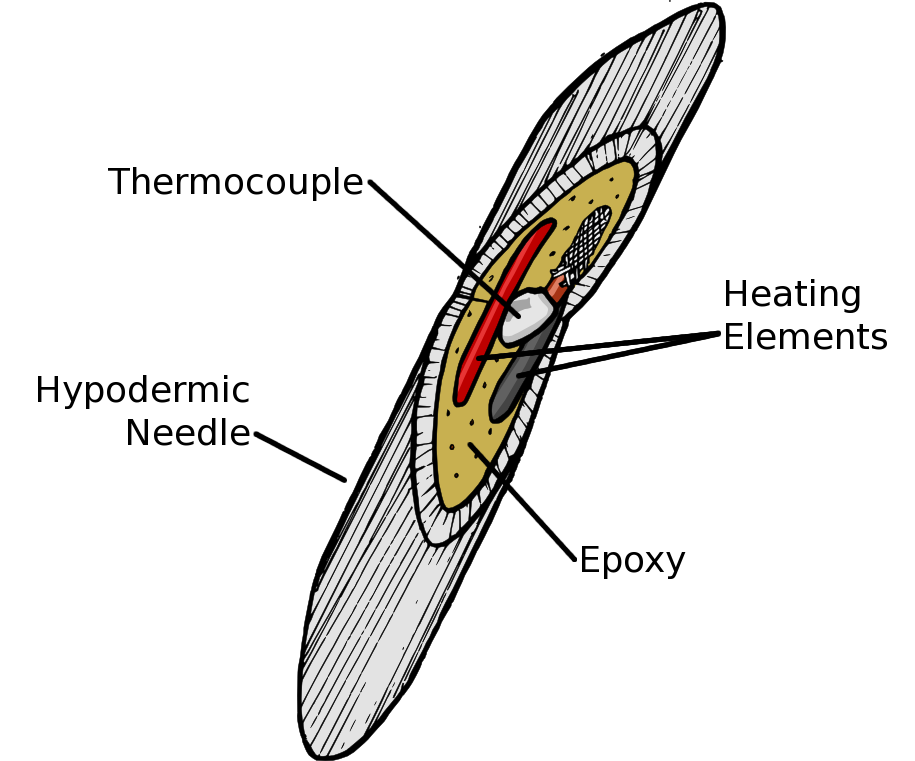
\includegraphics[width=0.8\textwidth]{fig/needle_xsect.png}
\end{columns}
\end{frame}


\begin{frame}
\frametitle{How Do You Measure \emph{Isotropic} Thermal Conductivity With It?}

\begin{columns}[c]
\column{0.3\textwidth}
    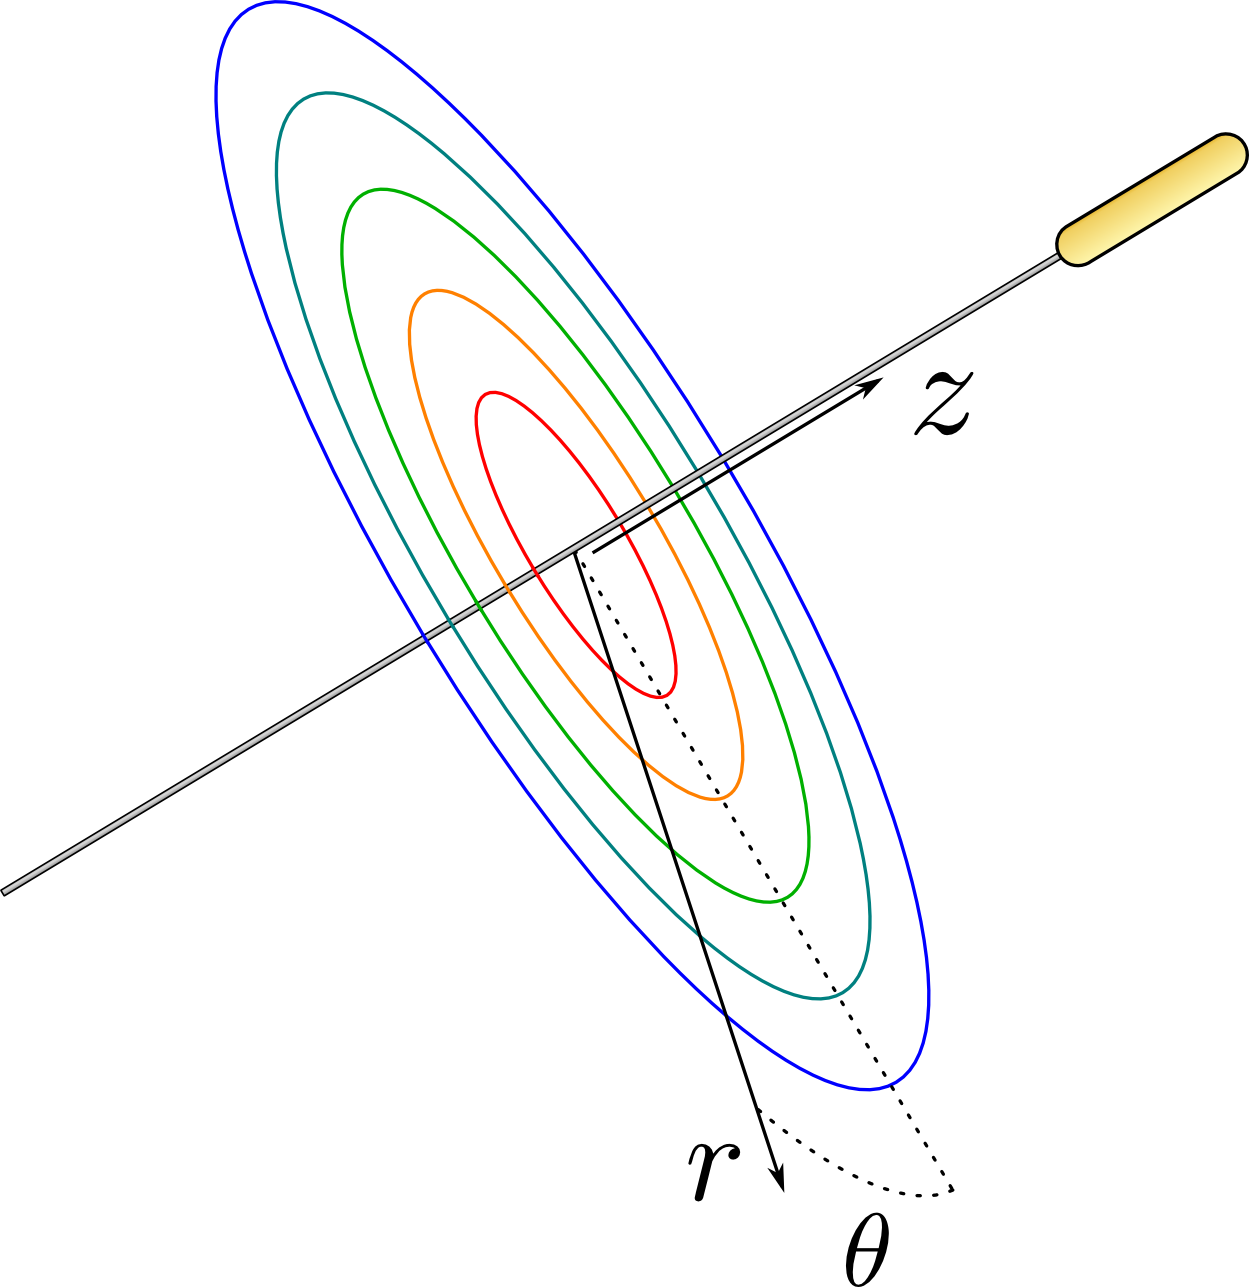
\includegraphics[width=\textwidth]{fig/basic_geometry.png}
\column{0.7\textwidth}
    \begin{enumerate}
    \item Write down The Heat Equation (\( -k\nabla^2 T = \rho C\frac{\partial T}{\partial t} \) in 3D Cartesian coordinates---Note the constant \(k\)
    simplification).
    \item Pose your problem in cylindrical coordinates, with constant heat flux at \(z=0\)
    \item Find a book where somebody has solved it for you already
    (Carslaw \& Jaeger) and write down the solution:

    \begin{equation*}
    T(r,t) = -\frac{q}{4\pi k}\Ei\left(-\frac{r^2}{4kt}\right)
    \end{equation*}

    \end{enumerate}
\end{columns}
\end{frame}


\begin{frame}
\frametitle{\(\Ei()\)? What's \emph{that}?}

\[\Ei(x) = -\int_{-x}^{\infty} \frac{e^{-t}}{t}dt \]

\begin{itemize}
\item ...in \emph{this} case. Some people define it differently.
\item You can't do that integral analytically, unfortunately.
\item \emph{However}, there \emph{are} long-time, small-radius approximations.
Hooray!
\end{itemize}
\end{frame}


\begin{frame}
\frametitle{Useful Approximation Action}

Over time, the solution approaches this:

\begin{equation*}
T(r,t) = \frac{q}{4\pi k}\ln\left(\frac{4kt}{r^2}\right) - \frac{\gamma q}{4\pi k}
\end{equation*}

But, more usefully:

\begin{equation*}
\frac{\partial T}{\partial \ln(t)} = \frac{q}{4\pi k}
\end{equation*}

\end{frame}


\begin{frame}
\frametitle{Finding Conductivities: A Real-Life Example}

This is a temperature/time curve for an actual measurement of snow behind my
house:

\begin{columns}[c]
\column{0.6\textwidth}
    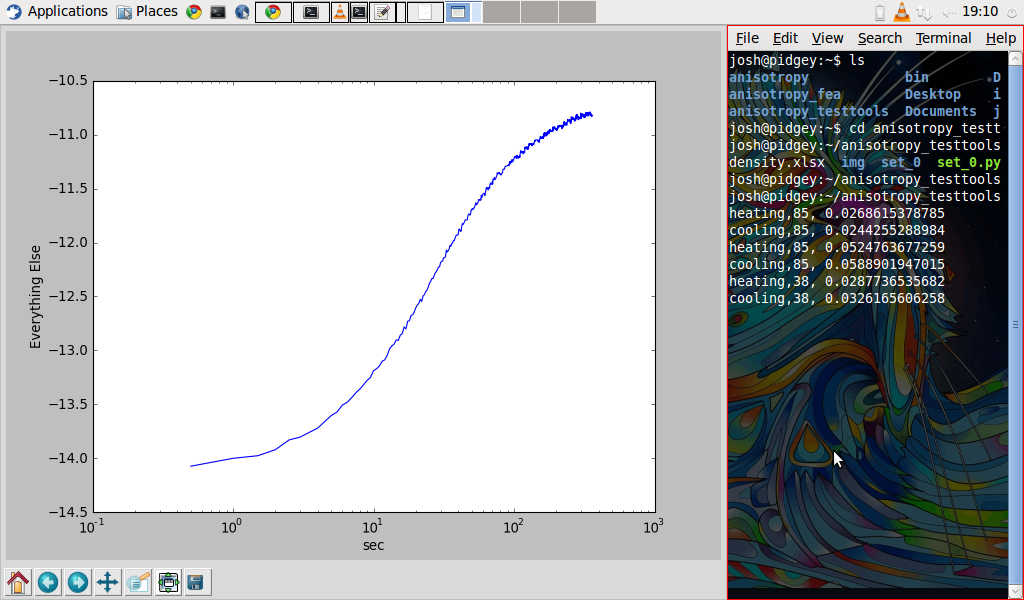
\includegraphics[width=\textwidth]{fig/measurement_graph.png}
\column{0.4\textwidth}
    \begin{itemize}
    \item Early ``transient'' behavior (The whole situation's transient conduction)
    \item Mid-range, steady-slope behavior (This is what we're interested in)
    \item Late-game in-snow convection (Can be mitigated by using less heat)
    \end{itemize}
\end{columns}
\end{frame}


\begin{frame}
\frametitle{There's a Cooling Curve, As Well}
\begin{itemize}
\item That was what's called the ``heating curve.''
\item The ``cooling curve'' is when you watch the needle cool back down.
\item By an analogous derivation, we can find a similar long-time solution for
cooling curve slope over \(\ln(t_{\textrm{cooling}})\)
\item Used in measurements, but not modeled. Sorry, guys.
\end{itemize}
\end{frame}


\begin{frame}
\frametitle{Metamorphic Powder Rangers: How Snow Becomes Anisotropic}
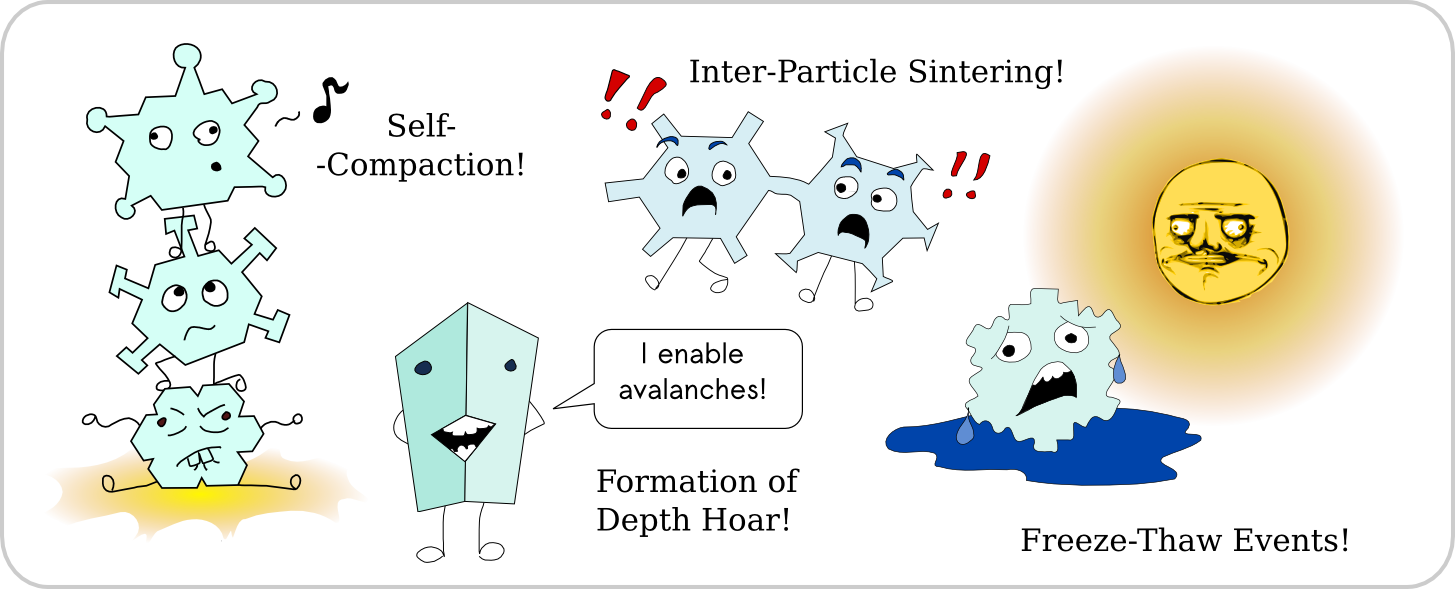
\includegraphics[width=\textwidth]{fig/metamorphism.png}\\
These processes cause snow to form regions of varying thermal conductivity---for
example, alternating layers of high and low conductivity.
\end{frame}


\begin{frame}
\frametitle{Example Time!}
\begin{columns}[c]
\column{0.5\textwidth}
    \centering
    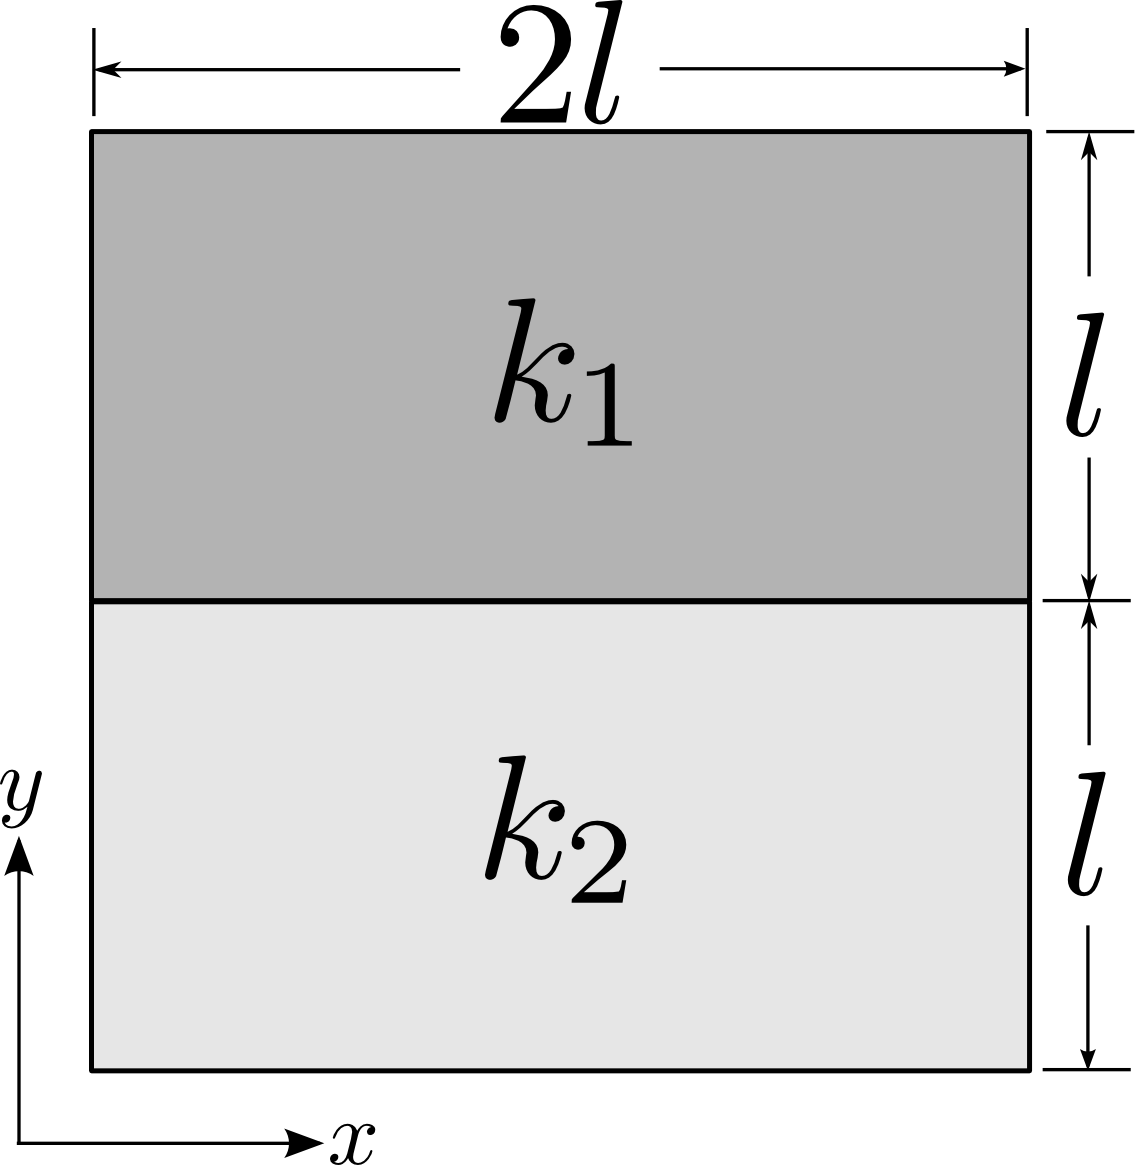
\includegraphics[width=0.7\textwidth]{fig/ex_laminate.png}
\column{0.5\textwidth}
    \begin{itemize}
    \item Vertically: \(\frac12(k_1 + k_2)\)
    \item Horizontally: \(2\left( \frac1{k_1} + \frac1{k_2} \right)^{-1}\)
    \end{itemize}
\end{columns}
\smallskip
Keep this example in mind for later!
\end{frame}

\begin{comment}
Note: We can also discuss some of the questions being brought up, but I'd like
to Broad Overview this.
\end{comment}

\begin{frame}
\frametitle{The Basic Model}
\begin{columns}[c]
\column{0.4\textwidth}
    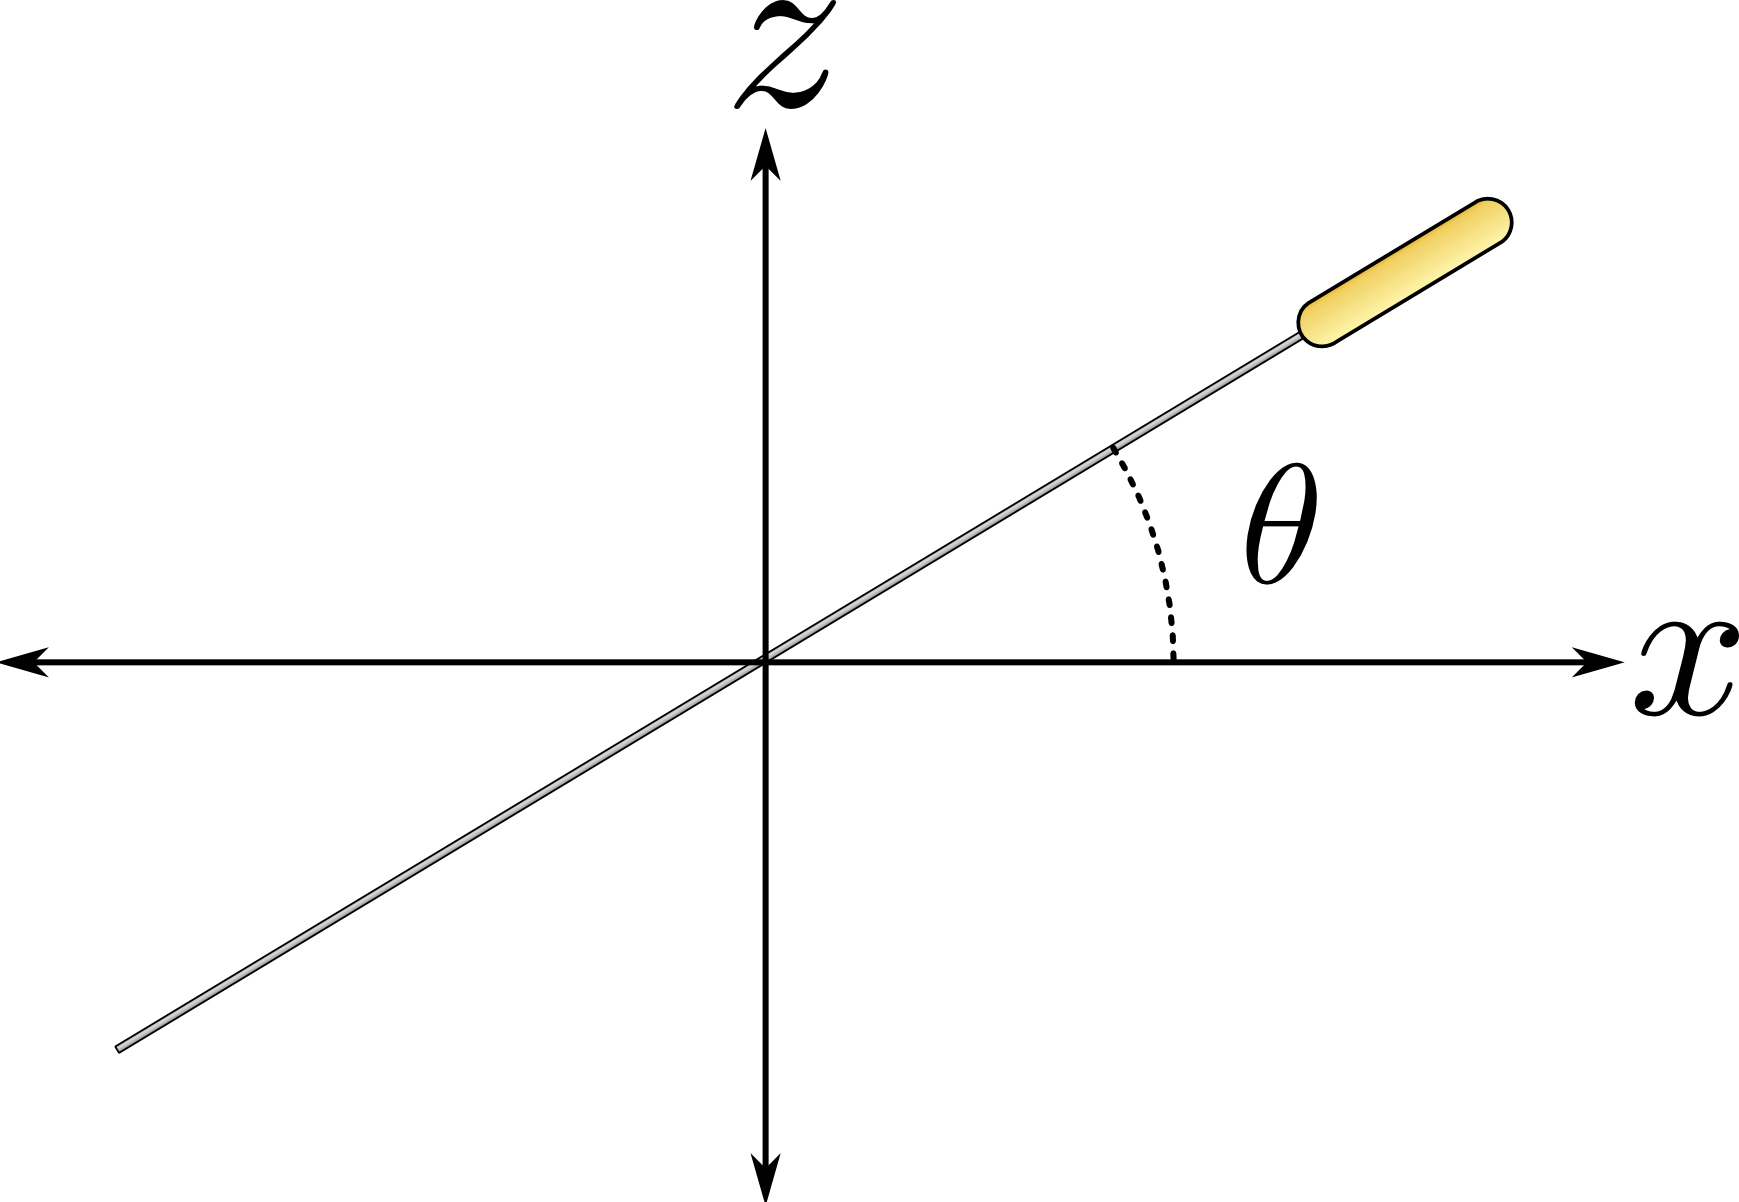
\includegraphics[width=\textwidth]{fig/angle.png}
\column{0.6\textwidth}
    \begin{itemize}
    \item Horizontal and Vertical conductivities only.
    \item Needle rotated from the horizontal.
    \item Goal: Find \(k_{\textrm{meas}}(\theta)\) for a given \(k_{xy}\) and \(k_z\).
    \end{itemize}
\end{columns}
\end{frame}


\begin{frame}
\frametitle{Outline!}
\begin{itemize}
\item Analytical Approaches
\item Numerical Modeling in COMSOL
\item Measurements of Snow and Engineered Materials
\item Results
\item Loose Ends
\end{itemize}
\end{frame}


\begin{frame}
\frametitle{Analytical Approaches}
\begin{columns}[c]
\column{0.5\textwidth}
    \begin{itemize}
    \item We already have a working isotropic theory
    \item But for the anisotropic case, the conductivity is a \(3\times 3\), positive definite matrix!
    \item Can we adapt the isotropic theory to the anisotropic cases? (Yes.)
    \end{itemize}
\column{0.5\textwidth}
    \begin{equation*}
    \nabla \cdot \begin{bmatrix}
    k_{11} & k_{12} & k_{13}\\
    k_{12} & k_{22} & k_{23}\\
    k_{13} & k_{23} & k_{33}
    \end{bmatrix}\nabla T = -\rho C\frac{\partial T}{\partial t}
    \end{equation*}
\end{columns}
\end{frame}


\begin{frame}
%That texttt mess is for making the dashes not blend.
\frametitle{First: \texttt{dimension-}\texttt{-;}}
\centering
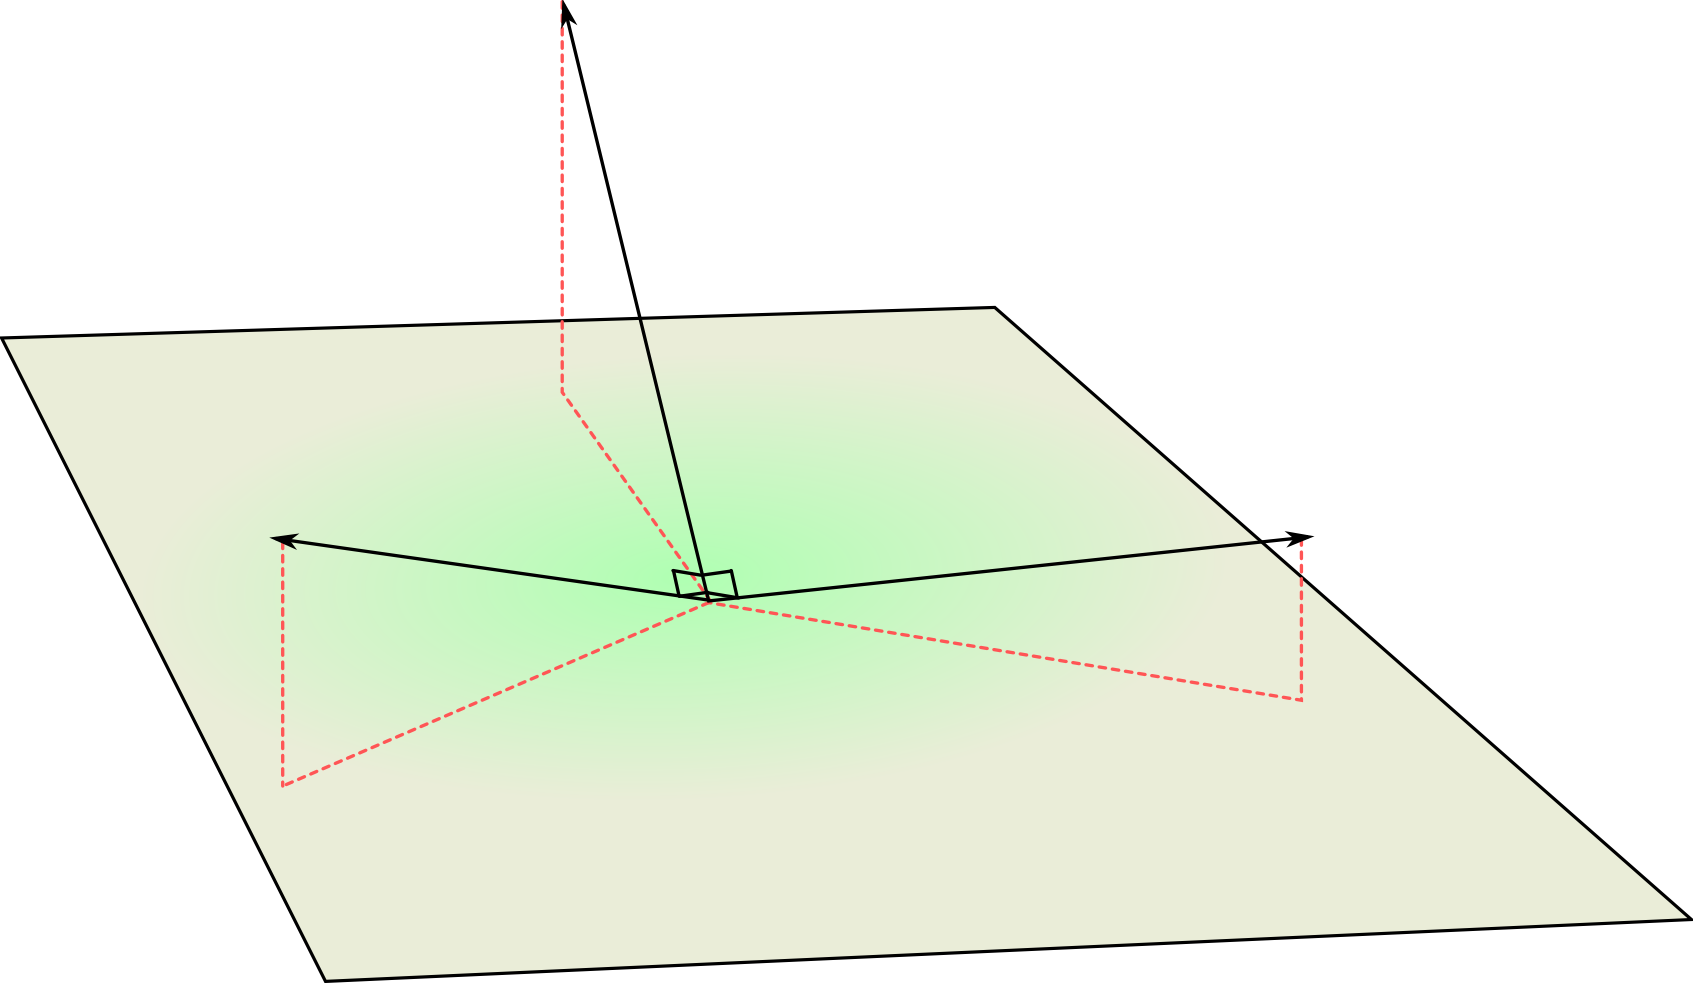
\includegraphics[width=0.6\textwidth]{fig/projection.png}
\begin{itemize}
\item Remember, there's no temperature gradient in the \(z\) direction!
\item First, drop the \(z\) coordinates, then find the positive eigenvalues.
\end{itemize}
\end{frame}

\begin{frame}
\frametitle{Second: Stretch!}
We now have:
\begin{equation*}
-\nabla \cdot \left(\begin{bmatrix}k_x & 0\\ 0 & k_y\end{bmatrix}\nabla T \right)= \rho C\frac{\partial T}{\partial t}
\end{equation*}

\begin{columns}
\column{0.5\textwidth}
    \begin{itemize}
    \item What if we use a different coordinate system (\(x'\) and \(y'\)) to make
    that matrix a multiple of \([I]\)?
    \end{itemize}
\column{0.5\textwidth}
    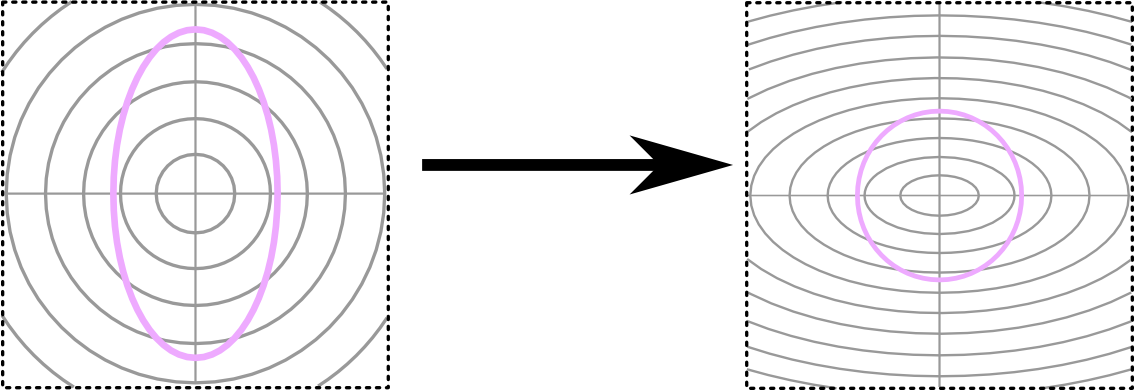
\includegraphics[width=\textwidth]{fig/coordinate_transformation.png}
\end{columns}
\end{frame}

\begin{frame}
\frametitle{Math Alert! Math Alert!}

\begin{align*}
x' &= a_x x\\
y' &= a_y y\\
a_x &= 1 \textrm{ (WLOG)}
\end{align*}
\begin{align*}
\frac{dx'}{dx} &= 1\\
\frac{dy'}{dy} &= a_y
\end{align*}
\end{frame}


\begin{frame}
\frametitle{It's Not Over Yet.}
\begin{align*}
\frac{\partial f}{\partial x} &= \frac{\partial f}{\partial x'}\frac{dx'}{dx} = \frac{\partial f}{\partial x'}\\
\frac{\partial f}{\partial y} &= \frac{\partial f}{\partial y'}\frac{dy'}{dy} = a_y\frac{\partial f}{\partial y'}
\end{align*}

\begin{align*}
\nabla T &= \frac{\partial T}{\partial x'} \e_{x'} + a_y\frac{\partial T}{\partial y'} \e_{y'} \\
[K]\nabla T &= k_x\frac{\partial T}{\partial x'} \e_{x'} + k_ya_y\frac{\partial T}{\partial y'} \e_{y'}\\
\nabla \cdot \left([K]\nabla T\right) &= k_x\frac{\partial^2 T}{\partial {x'}^2} + k_ya_y^2\frac{\partial^2 T}{\partial {y'}^2}\\
\end{align*}
\end{frame}


\begin{frame}
\frametitle{Almost Done!}
Suppose the right hand side is equal to the equivalent isotropic expression:
\begin{equation*}
k\left(\frac{\partial^2 T}{\partial {x'}^2} + \frac{\partial^2 T}{\partial {y'}^2} \right) = k_x\frac{\partial^2 T}{\partial {x'}^2} + k_ya_y^2\frac{\partial^2 T}{\partial {y'}^2}
\end{equation*}

THIS MEANS:

\begin{align*}
k &= k_x\\
a_y &= \sqrt{\frac{k_x}{k_y}}
\end{align*}
\end{frame}

\begin{frame}
\frametitle{But Then, A Shocking Twist.}
\begin{equation*}
T(r',t) = \frac{q}{4\pi k_x}\ln\left(\frac{4k_xt}{r'^2}\right) - \frac{\gamma q}{4\pi k_x}
\end{equation*}
\begin{itemize}
\item This equation is in terms of \(r'\), not \(r\)!
\item If you try to take your derivative here, it \emph{will not work like you want it to}.
\item We need to do something with the \(r'\) this time.
\end{itemize}
\end{frame}


\begin{frame}
\frametitle{What Is \(r\) \emph{Anyway?}}
\begin{itemize}
\item Arguably, our Actual Measurement is the average temperature at some finite 
\(r\) from the center of the needle.
\item There are other approaches one may take, such as assuming a non-zero needle
thickness in the problem formulation.
\item It can be shown (as it is in the thesis) that:
\begin{equation*}
    \norm{r'}^2 = r_0^2 \left(\cos^2(\theta) + \frac{k_x}{k_y}\sin^2(\theta) \right)
\end{equation*}
\item Note, \(r'\) is a function of \(\theta\).
\end{itemize}
\end{frame}


\begin{frame}
\frametitle{Elliptical Integral Time}
\begin{itemize}
\item Taking the averaging approach, our problem can now be described as so:
\begin{equation*}
T_{\textrm{avg}}(t) = \frac{4\pi k_x}{q} \frac{\mathcal{E}(\ln(t), \frac{k_y}{k_x})}{\mathcal{E}(1, \frac{k_y}{k_x})}
\end{equation*}

\item What's this \(\mathcal{E}\) stuff?
\begin{equation*}
\mathcal{E}(f(\phi, \alpha), \alpha) = \int_0^{2\pi} f\sqrt{\cos^2(\phi) + \alpha\sin^2(\phi)} d\phi
\end{equation*}
\item Curve fit \emph{this} equation to the \(T = A \ln(t) + C\) form, and you now
have a \(k_{\textrm{meas}}\)!
\end{itemize}
\end{frame}


\begin{frame}
\frametitle{Implementation Notes}
\begin{itemize}
\item I used python and numpy/scipy.
\item Integrals are evaluated numerically using a quadrature method.
\item Source available upon request.
\end{itemize}
\end{frame}


\begin{frame}
\frametitle{Numerical Modeling!}
\begin{columns}[c]
\column{0.4\textwidth}
    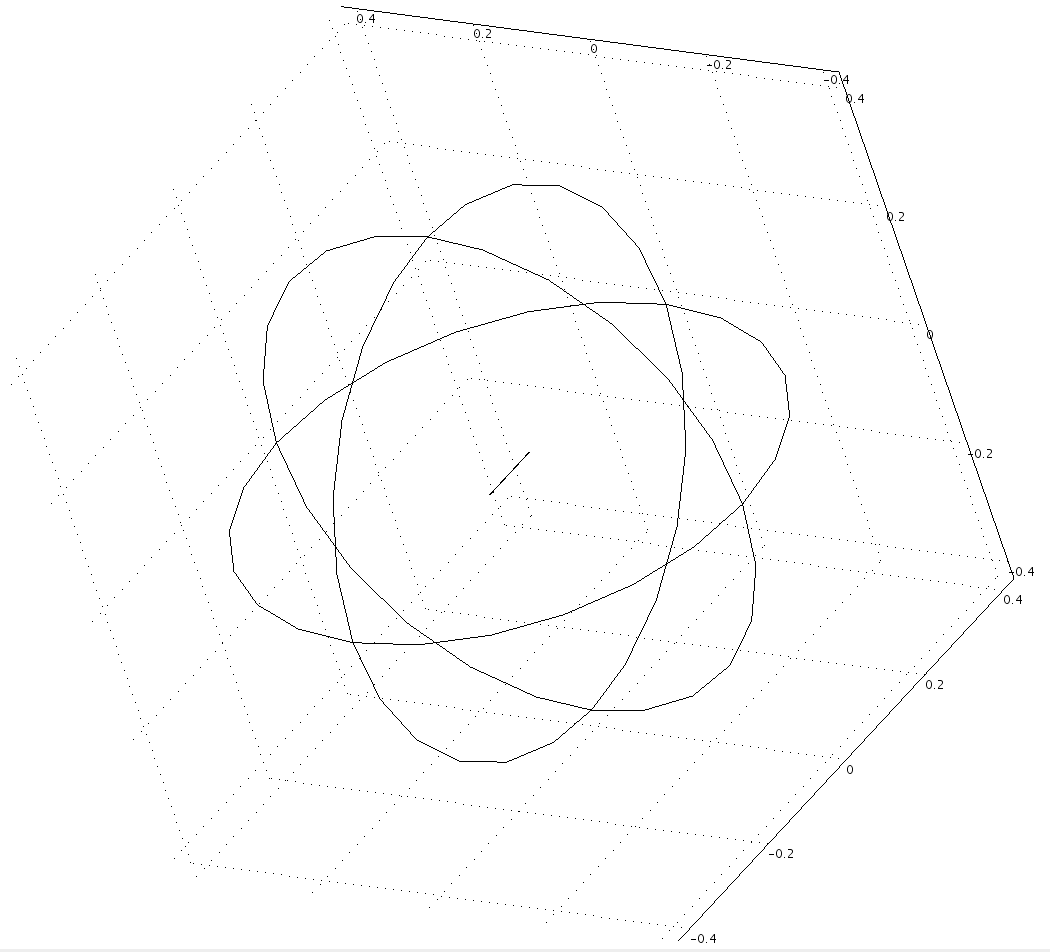
\includegraphics[width=\textwidth]{fig/domain.png}
\column{0.6\textwidth}
    \begin{itemize}
    \item 3D Model in COMSOL 3.5a
    \item Steel needle embedded in sphere \emph{*cough*}snow\emph{*cough*}
    \item Yes, that's a sphere.
    \item ``Wait! This medium's not infinite!'' \begin{itemize}
        \item It's \emph{pretty big} compared to the needle
        \item Zero heat flux boundary conditions on the sphere
        \item Monitored temperatures on the boundary showed O(\(10^{-14}\)) degrees in change, so it's ``big enough.''
        \end{itemize}
    \end{itemize}
\end{columns}
\end{frame}


\begin{frame}
\frametitle{Constant Parameters}
\begin{table}
\centering
\begin{tabular}{r | l}
radius of needle & \(0.25\) mm\\
length of needle & \(10\) cm\\
radius of snow & \(40\) cm\\
\hline
density of needle & \(8000\) kg/\(\textrm{m}^3\)\\
\(C_P\) of needle & \(460\) \(\flatfrac{\textrm{J}}{\textrm{kg}\cdot\textrm{K}}\) \\
\(q\) of needle & \(0.5\) W/m\\
\(k\) of needle & \(160\) W/m\(\cdot\)K\\
\hline
density of snow & \(200\) kg/\(\textrm{m}^3\)\\
\(C_P\) of snow & \(2050\)  \(\flatfrac{\textrm{J}}{\textrm{kg}\cdot\textrm{K}}\)
\end{tabular}
\end{table}
\end{frame}


\begin{frame}
\frametitle{Rotating The Domain (Easier Than Rotating The Needle)}
    \begin{equation*}
    K = \begin{bmatrix}
    \cos(\theta) & 0 & \sin(\theta)\\
    0 & 1 & 0\\
    -\sin(\theta) & 0 &\cos(\theta)
    \end{bmatrix}
    \begin{bmatrix}
    k_{xy} & 0 & 0\\
    0 & k_{xy} & 0\\
    0 & 0 & k_z
    \end{bmatrix}
    \begin{bmatrix}
    \cos(\theta) & 0 & \sin(\theta)\\
    0 & 1 & 0\\
    -\sin(\theta) & 0 &\cos(\theta)
    \end{bmatrix}
    \end{equation*}
    \begin{itemize}
    \item Instead of rotating the needle, we rotate the planes of anisotropy.
    \item Both approaches work, but COMSOL handles arbitrary \(K\) better than
          changes in domain geometry.
    \item That means it crashes less.
    \end{itemize}
\end{frame}


\begin{frame}
\frametitle{``Parameter Studies,'' COMSOL and MATLAB}
\begin{itemize}
\item COMSOL 3.5 doesn't have built-in facilities for complex parameter studies
(COMSOL 4.1 is better!)
\item However, there \emph{are} MATLAB bindings for scriptage
\item Good to go!
\end{itemize}
\end{frame}


\begin{frame}
\frametitle{Program Structure}
\begin{itemize}
\item mesher.m does the meshing
\item solver.m does the solving
\item fitter.m does the curve-fitting
\item worker.m does the bossing around
\item Master m-file and a bash command tell the worker what to do
\end{itemize}
\end{frame}


\begin{frame}
\frametitle{mesher.m}
\begin{columns}[c]
\column{0.4\textwidth}
    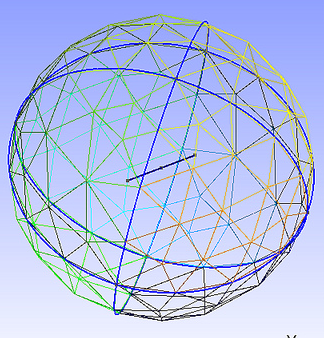
\includegraphics[width=\textwidth]{fig/example_mesh.png}
\column{0.6\textwidth}
\begin{itemize}
    \item Mostly auto-generated code, wrapped in a function call
    \item Assigns geometry parameters (lengths, widths, etc.)
    \item Generates a mesh to do the solving on
    \item Returns ``fem'' structure
    \end{itemize}
\end{columns}
\end{frame}


\begin{frame}
\frametitle{solver.m}
\begin{itemize}
\item Also mostly auto-generated and ``function-ized''
\item Takes fem object from mesher as an argument
\item Assigns material properties (conductivity, heat capacity, etc.)
\item Solves the problem
\item Returns \((T,t)\) data for center of probe and averaged final temperature on 
cardinal surface points
\end{itemize}
\end{frame}


\begin{frame}
\frametitle{fitter.m}
\begin{itemize}
\item Find straight portion by finding maximum number of consecutive ``samples''
from the tail-end that are sufficiently straight
\item Used correlation coefficient as a measure of ``straightness''
\item This only works in idealized simulations, not in real life. Simulations don't mess up.
\end{itemize}
\begin{center}
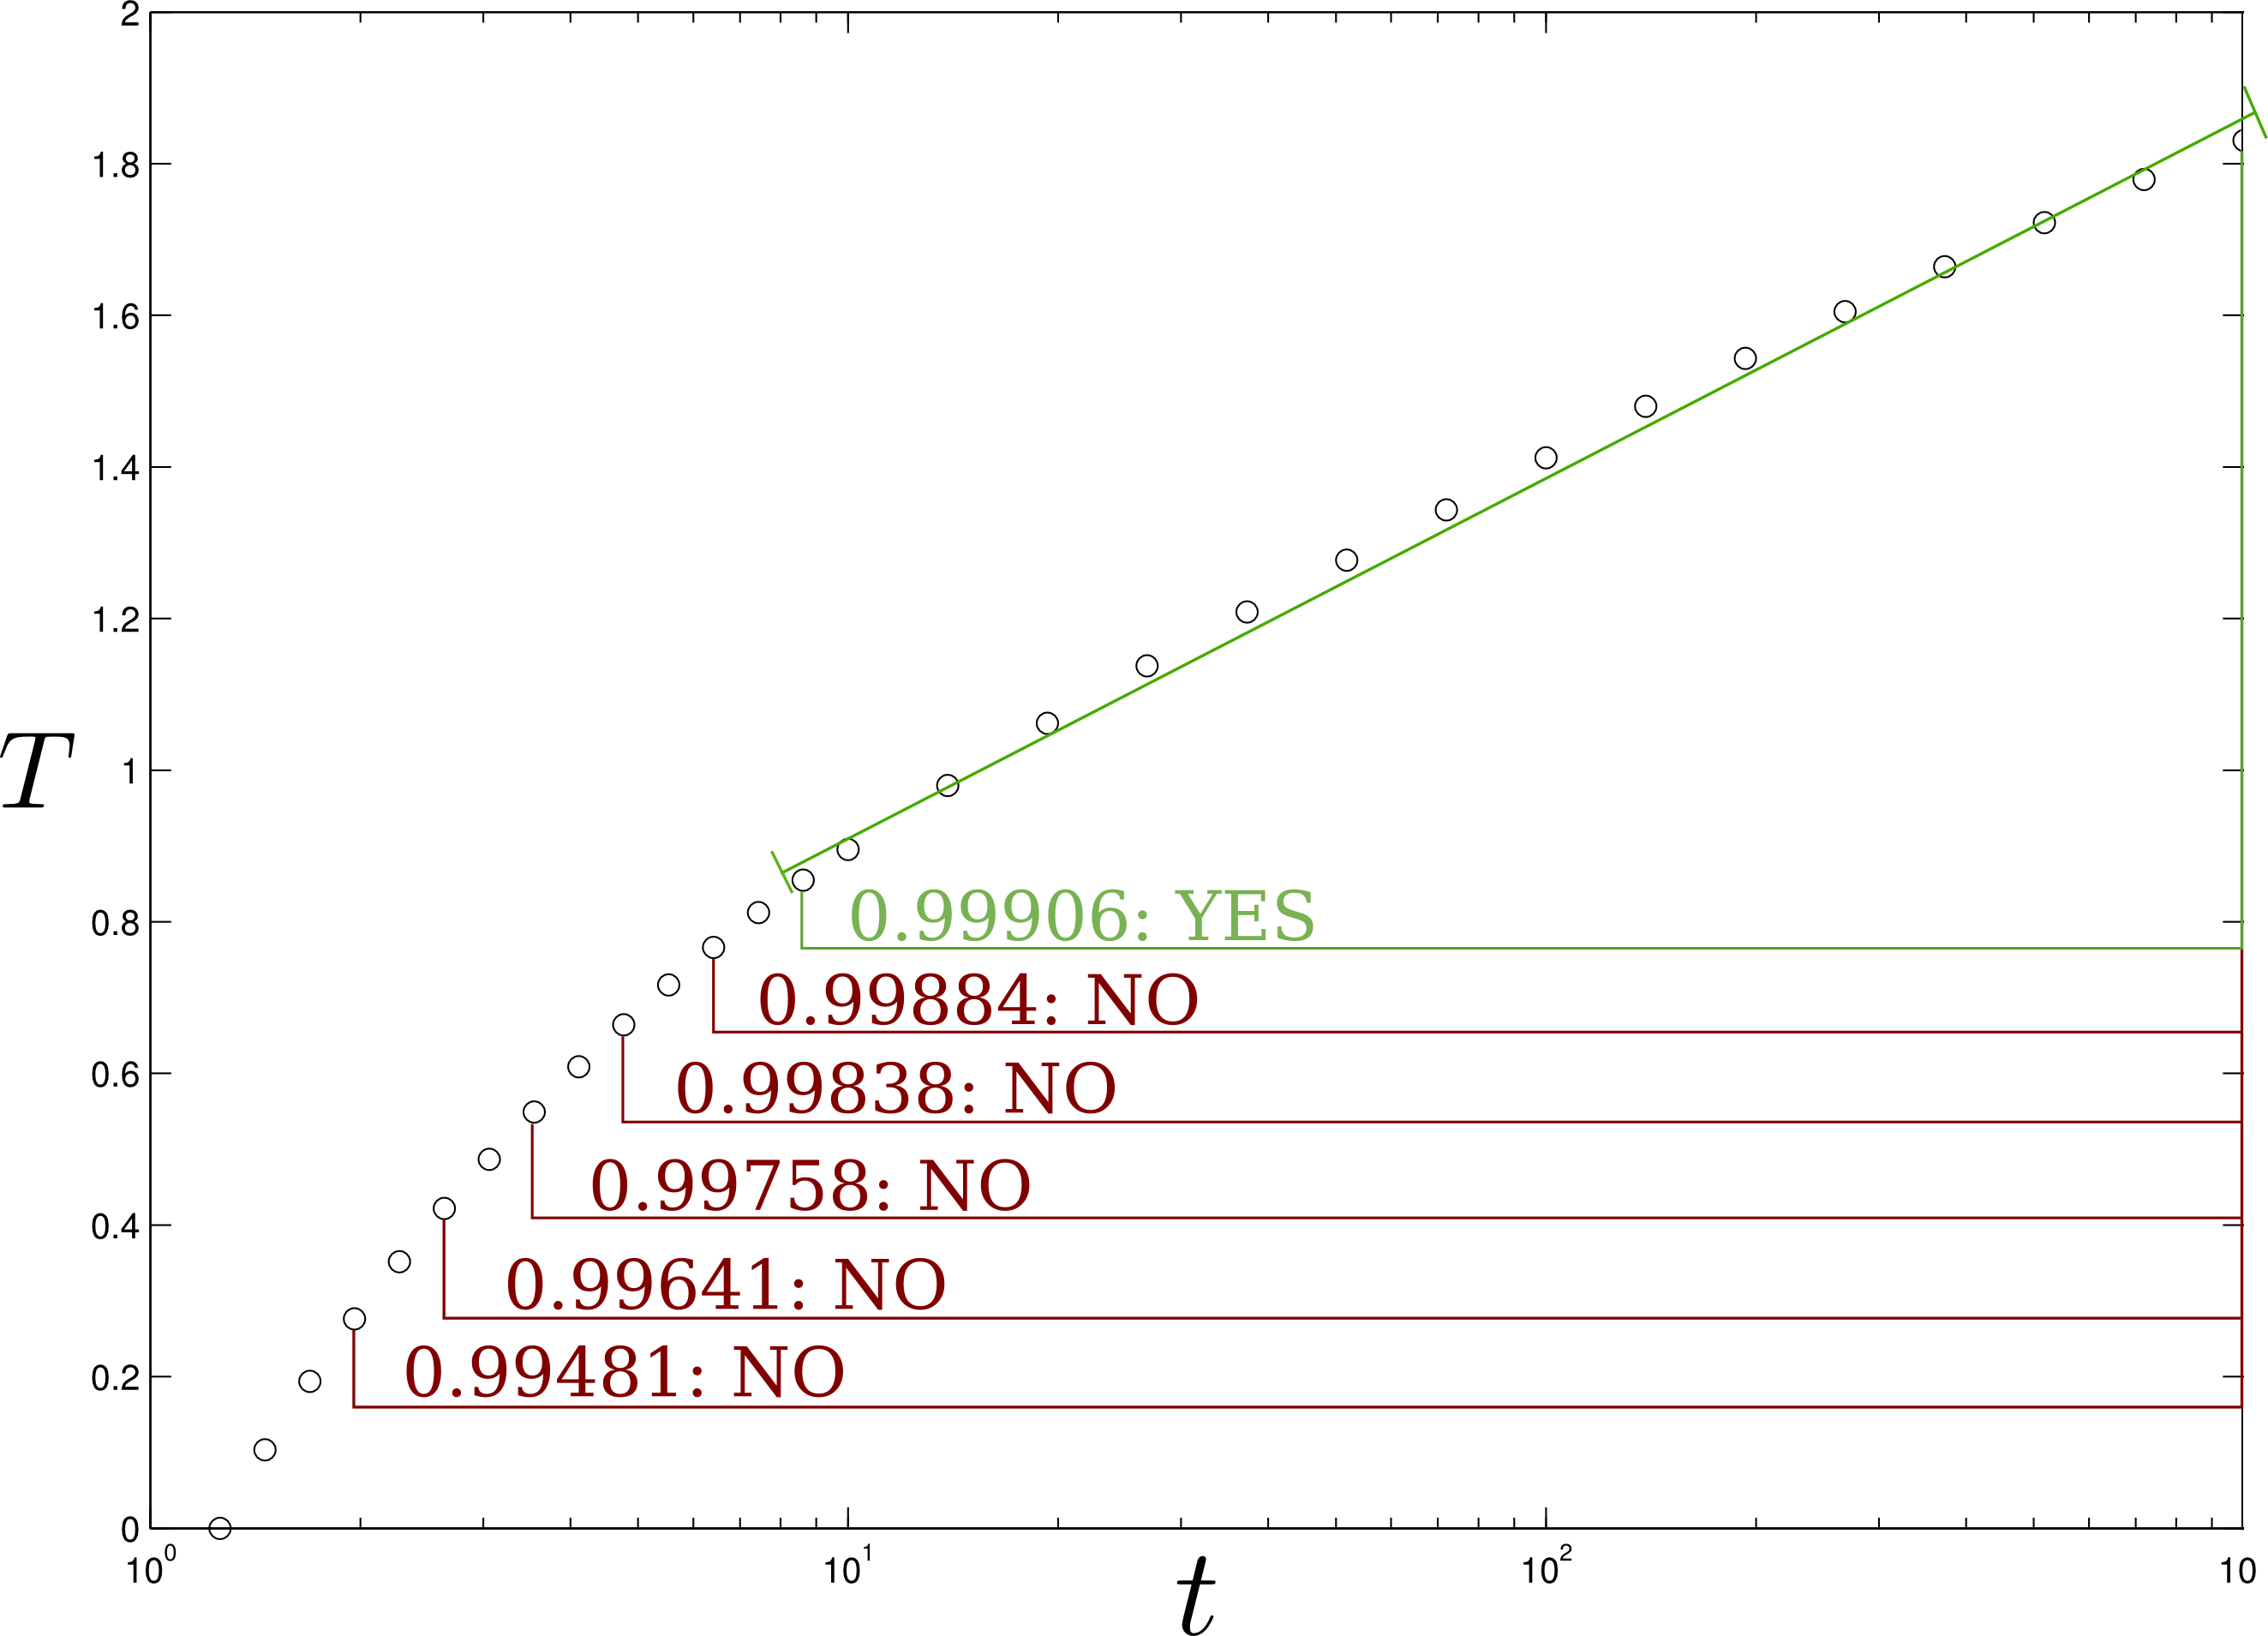
\includegraphics[width=0.6\textwidth]{fig/curvefit.png}
\end{center}
\end{frame}


\begin{frame}
\frametitle{worker.m}
\begin{itemize}
\item Stores solved data for every angle on-disk
\item Stores list of unsolved angles on-disk
\item Uses mapping functions over lists of \(k_{xy}\) and \(k_z\) meshgrids to
apply solver and fitter to varying situations
\item Combined with ``while :; do'' loop in bash, restarts after crashes
\item Only recovers by-angle, can not recover half-solved k-value combination sets.
\end{itemize}
\end{frame}


\begin{frame}
\frametitle{Resulting Data Structure}
\begin{itemize}
\item 2-D Cell Array (more like arrays in other languages than MATLAB's matrices/vectors) with indexes corresponding to \(k_{xy}\) and \(k_z\) MATLAB vector indices
\item Each ``slot'' in this cell array is \emph{another} cell array.
\end{itemize}
\begin{table}
\begin{tabular}{| c | c | c |}
\hline
\(k_\textrm{meas}\) & \( \left[ \textrm{time}, \textrm{temperature} \right]^T\) & Avg. surface temp. of sphere\\
\hline
\end{tabular}
\end{table}
\end{frame}


\begin{frame}
\frametitle{Convergence Study}
\begin{itemize}
\item Goal: Show that the solution as a function of mesh size converges on a particular solution.
\item Why: Makes sure solution ``has meaning'' \& that mesh size is reasonable
\item A Problem: Increasing mesh size makes the problem \emph{harder}.
\end{itemize}
\end{frame}


\begin{frame}
\frametitle{Convergence Study Runtimes}
    \begin{table}
    \begin{tabular}{r | r | l}
     & Number of Elements & Time to Complete\\
    ``Classic'' & \(35892\) elements & \(\approx 10\) minutes\\
    ``Intermediate'' & \(159641\) elements & \(\approx 2\) hours\\
    ``Nightmare'' & \(528945\) elements & ??? (\(>3\) weeks)\\
    \end{tabular}
    \end{table}
\textbf{Q:} What the heck happened in ``Nightmare'' mode?

\textbf{A:}\\
\begin{center}
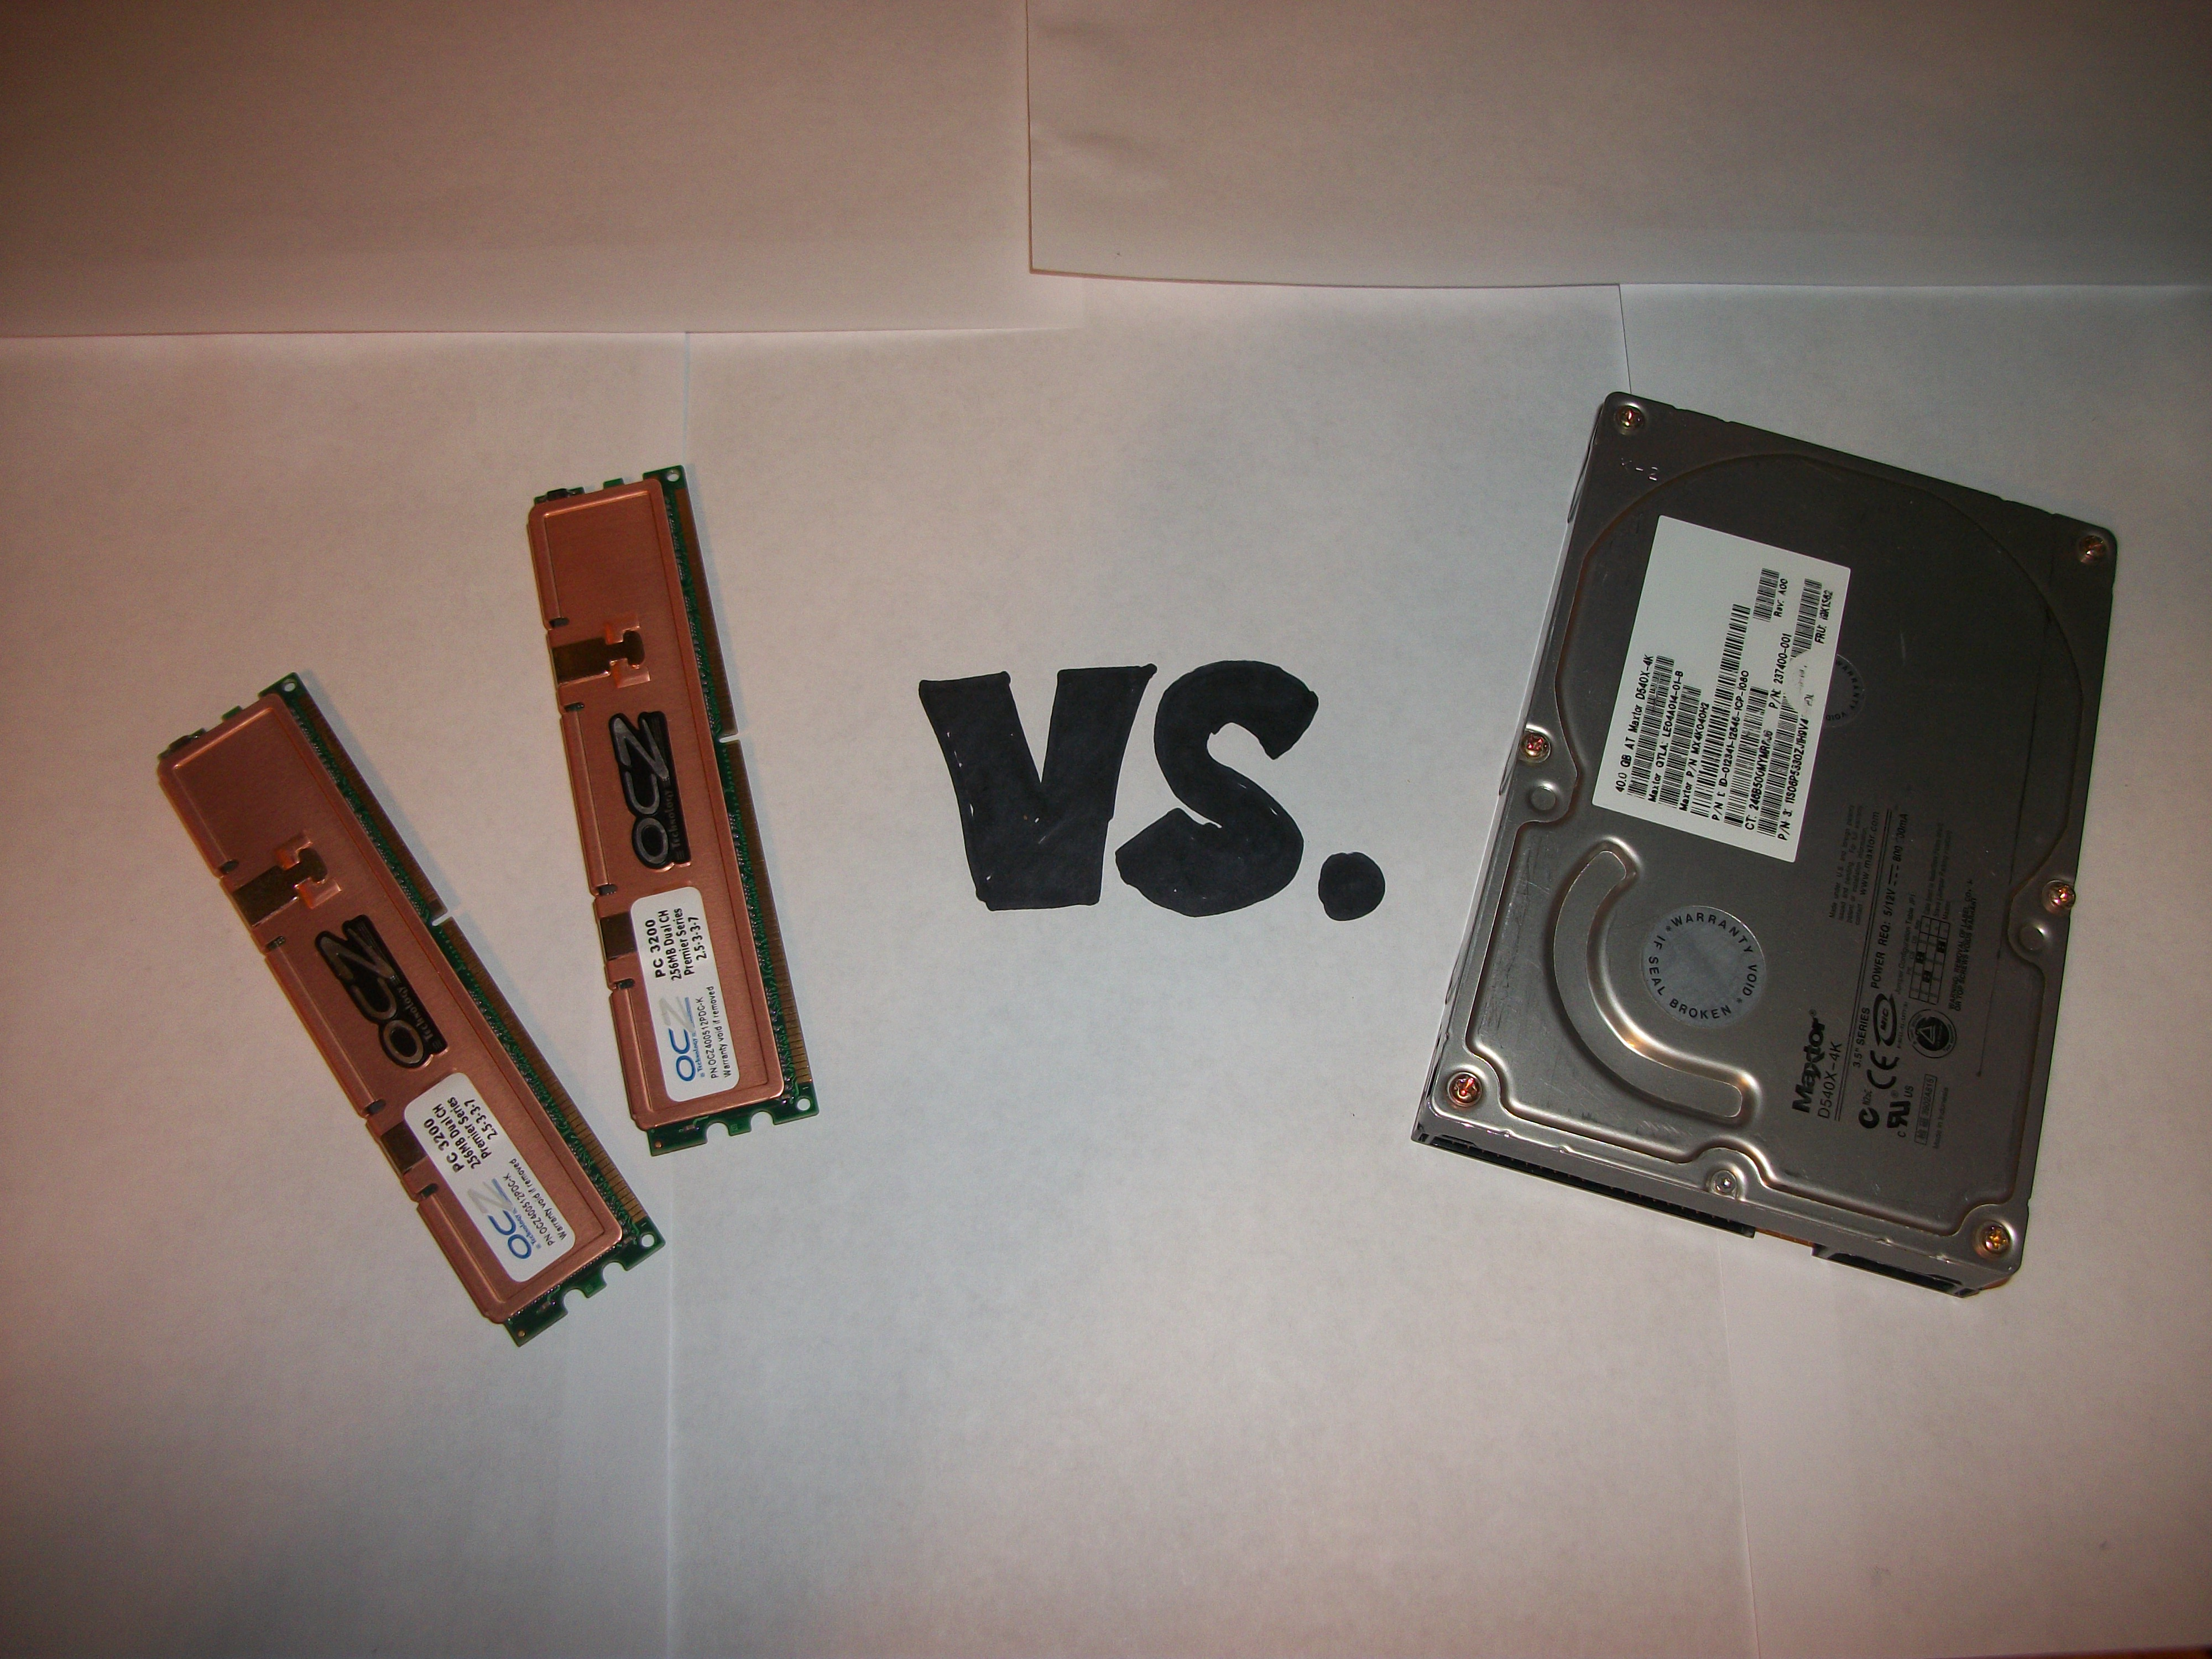
\includegraphics[width=0.4\textwidth]{fig/thedisk.jpg}
\end{center}
\end{frame}


\begin{frame}
\frametitle{Needle Probe Fundamentals}
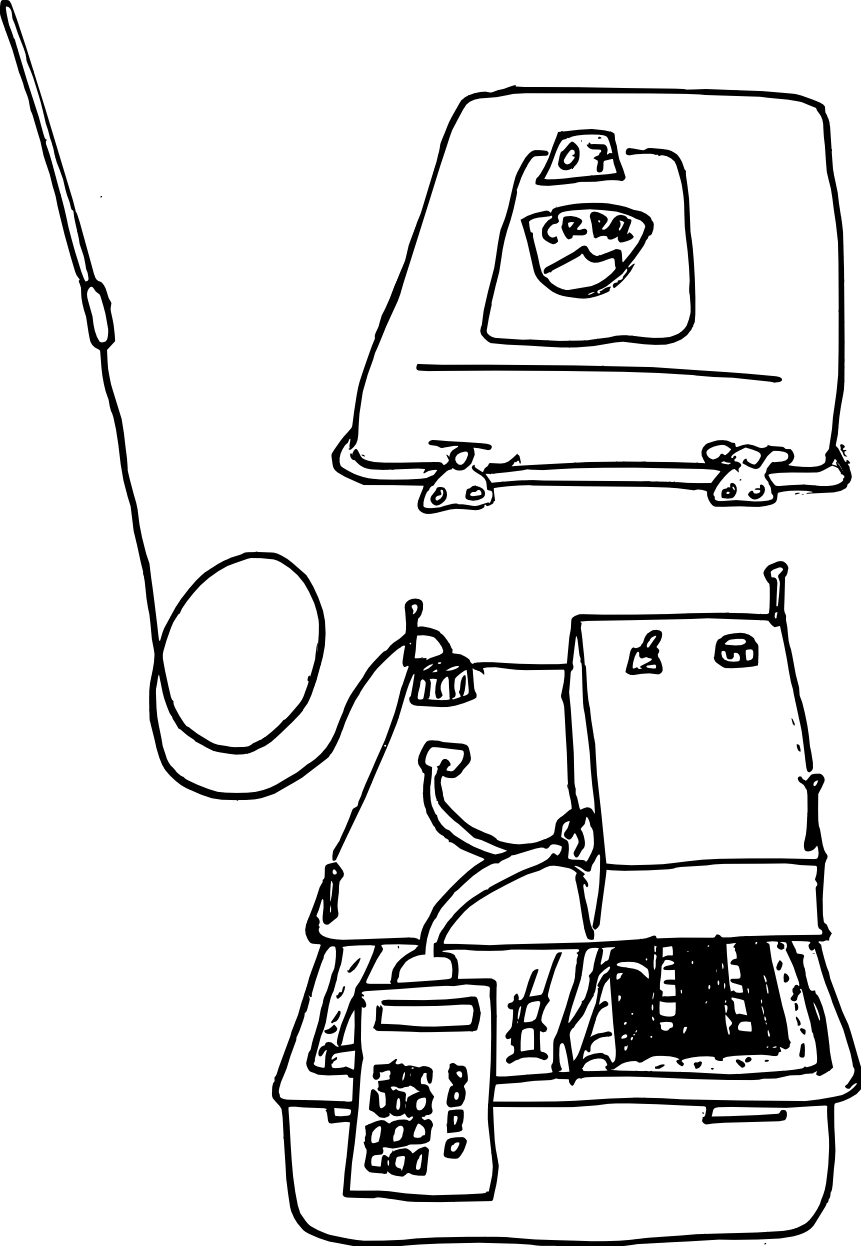
\includegraphics[width=0.9\textwidth]{fig/apparatus.png}
\end{frame}


\begin{frame}
\frametitle{How To Use:}
\begin{enumerate}
\item Turn on the device.
\item Insert the needle into medium being measured.
\item Turn on the first register by pressing ``* 6 A D 1''. This makes the
apparatus measure temperature.
\item Turn on the second register by pressing ``* 6 A D 2''. This turns on the
heating element, effectively starting the test.
\item Wait 20 minutes for test to complete (5 min. heating, 10 min. cooling).
\end{enumerate}
\end{frame}


\begin{frame}
\frametitle{PC200W}
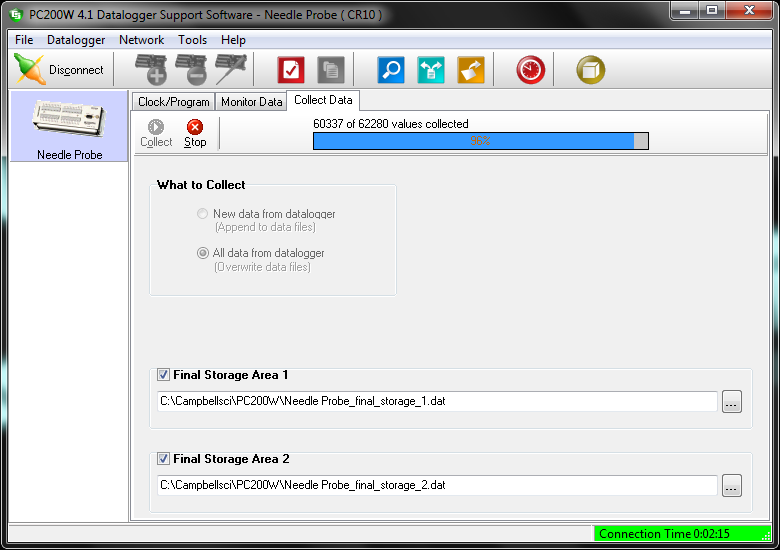
\includegraphics[width=\textwidth]{fig/pc200w.png}\\
You use this software to get data off the data logger and eventually convert it
to .csv format
\end{frame}


\begin{frame}
\frametitle{CSV Headers}
\begin{enumerate}
\item An instrument ID (constant in this case).
\item Ordinal day, out of 366. For example, March 17th is day 76.
\item hh:mm portion of timestamp. For example, 6:30pm is represented as 1830.
\item Seconds portion of timestamp.
\item Needle temperature, in Celcius.
\item Reference temperature, in Celcius.
\item Voltage across needle probe, in millivolts.
\item Experiment timer, in seconds.
\end{enumerate}
\end{frame}


\begin{frame}
\frametitle{Metadata}
\begin{itemize}
\item Each measurement has associated metadata (ie, angle) that is not kept
track of by the needle probe.
\item One must be careful to keep the right metadata associated with the right
time series!
\item I did this with folder structure, comments in calculation scripts, and associated .csv files.
\end{itemize}
\end{frame}


\begin{frame}
\frametitle{How do you measure angle, anyway?}
\begin{itemize}
\item A protractor and a plumb bob works \emph{okay}.
\item Simple, but with non-negligible error, especially in the case of snow.
\item Unimplemented alternative: 3-axis accelerometer (bonus points: compass bearing).
\end{itemize}
\end{frame}


\begin{frame}
\frametitle{PLEASE hand-inspect real-world measurements!}
\begin{center}
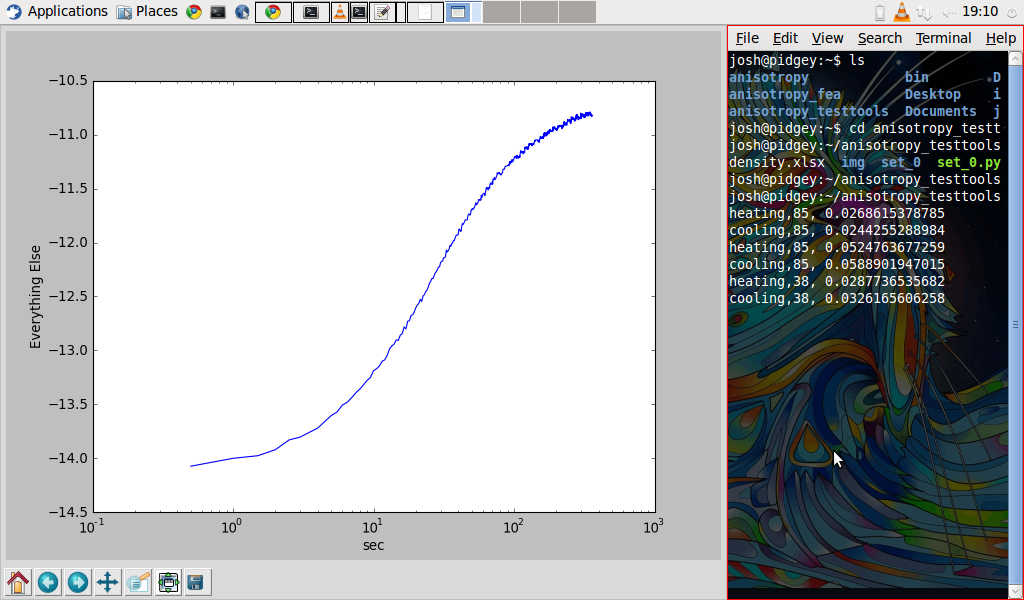
\includegraphics[width=\textwidth]{fig/measurement_screenie.png}
\end{center}
\end{frame}


\begin{frame}
\frametitle{Measuring Snow}
\begin{quotation}
  {\it ``It's non-trivial.''} \\ 
  \hspace*{1in}---Dr. Jerome Johnson
\end{quotation}
\begin{enumerate}
\item Cold wires can be difficult to work with.
\item Cold electronics can be difficult to work with.
\item Snow is fragile.
\item Snow does not behave as nicely as COMSOL models.
\end{enumerate}
\end{frame}


\begin{frame}
\frametitle{Also-Measured}
\begin{enumerate}
\item Height above soil (tape measure)
\item Density of snow in area being measured (cardboard cylinder \& scale)
\item This could have been done better.
\end{enumerate}
\end{frame}

\end{document}
